\newcommand{\bitbox}[3]{
  \filldraw[fill=#2!80!white,draw=black] (#1,0) +(-.2,-.2) rectangle ++(.2,.2);
  \draw (#1,0) node{#3};
}
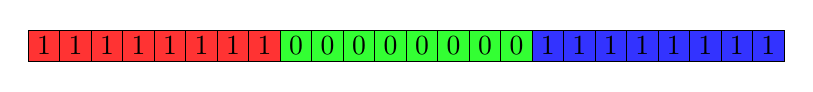
\begin{tikzpicture}
  \foreach \x in {-16.0,-15.6,...,-12.8}
  {
    \bitbox{\x}{red}{1}
  }
  \foreach \x in {-12.8,-12.4,...,-9.6}
  {
    \bitbox{\x}{green}{0}
  }
  \foreach \x in {-9.6,-9.2,...,-6.4}
  {
    \bitbox{\x}{blue}{1}
  }
\end{tikzpicture}
